\chapter{Edge impurity ion heating associated with m = 0 activity in PPCD}\label{ch:m0}

In addition to the more slow time scale ion thermal transport discussions, it is interesting to examine one particular phenomenon that is related to the improved confinement PPCD plasma, the m = 0 burst. Ideally, the m = 0 burst would not occur, and the datasets underlying the previous chapter are selected to avoid "bursty" PPCD shots. However, these m = 0 bursts and their heating effects are interesting subjects to study as they are relatively small perturbations, especially compared to the sawteeth events. Since they are brief events and the plasma returns to the PPCD quasi-equilibrium quickly, their effects can be more comfortably discussed as a perturbations on a (relatively) known state, as opposed to a perturbed-state in itself.  This section will first go into a brief discussion the current understanding of m = 0 bursts, their characteristics and their broader context in relation to PPCD plasmas. Then I discuss the measurements of impurity carbon heating observed in relation to theses bursts. Finally, I present the results modeling attempts within the framework of the ion thermal transport model discussed in previous chapters.

\section{Characteristics of m = 0 burst activity}
What is now called the m = 0 bursts were once referred to as "small dynamo events", especially in work revolving around the thesis of B. Chapman \cite{Chapman1997}. Similar to sawtooth events, the m = 0 bursts generates toroidal flux, and poloidal current. However, unlike the sawtooth events, they first appear in the edge resonant modes, in particular the m = 0 modes (hence it's current name). Despite it's current name, the m = 0 burst does excite the m = 1 tearing modes as well shortly after the m = 0 mode (see figure \ref{fig:m0_m_timing}), merely reversing the order of excitation as compared to sawtooth events. Further, it is not clear the the m = 0 bursts can be said to be caused by the destabilization of m = 0 modes, or that the m = 0 mode are themselves preceded by other instabilities. It is previous found that frequency of m = 0 bursts can be reduced by reversing $E_{\text{tor}}$ at the edge during the PPCD period, thereby help maintain the $E_\parallel > 0$\cite{Chapman2001}. Interestingly, the m = 0 bursts that persist in occurring after this optimization has been made are largely concentrated in the earlier part of the PPCD period, before edge $E_{\text{tor}}$ reverses (figure \ref{fig:m0_time}).

\begin{figure}
	\centering
	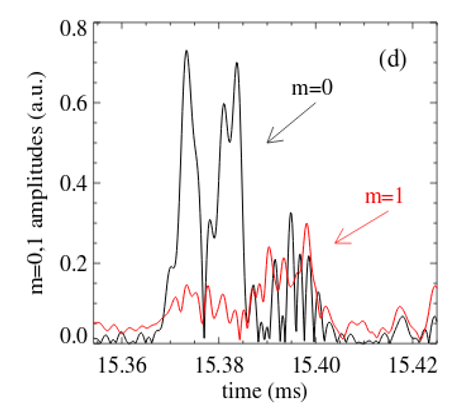
\includegraphics[width = 1.\linewidth]{./m0_and_impurity_heating/m0_timing.png}
	\caption[m = 0 vs m =1 mode amplitudes during m = 0 burst]{m = 0 vs m =1 mode amplitudes during m = 0 burst (Reproduced from Piovesean\cite{Piovesan2008})}\label{fig:m0_time}
\end{figure}

\begin{figure}
	\centering
	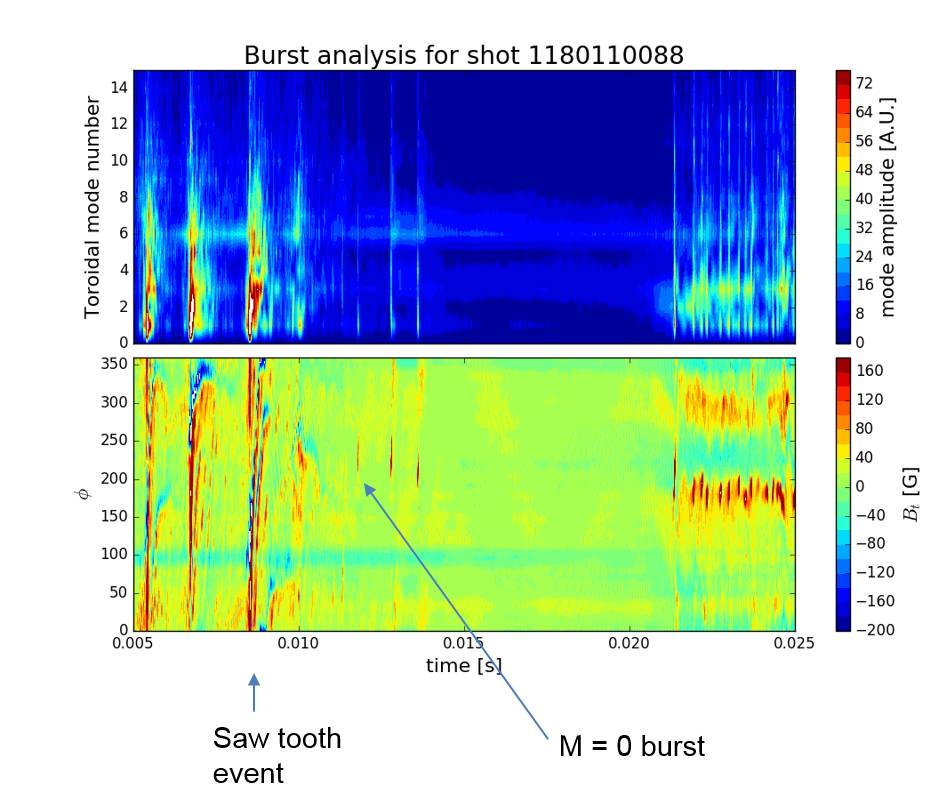
\includegraphics[width = 1.\linewidth]{./m0_and_impurity_heating/m0_example.png}
	\caption[Example mode and $B_t$ behavior]{Example of a typical bursty PPCD shot. The top presents a contour plot of the mode amplitudes vs time, broken down with respect to n number. On MST, m number break down is not always available but the n < 6 modes are m = 0 due to geometry constrains. The bottom presents a contour of the reconstructed $B_t$ values vs time and toroidal location ($\phi$). }\label{fig:m0_time}
\end{figure}

The m = 0 bursts involves a wide range of n numbers with coherent phase in such a way that it reconstructs to a single larger perturbation at one particular location, akin to the relation between a Dirac delta and it's Fourier transform. A good way to visualize some aspects of the m = 0 burst is presented in figure \ref{fig:m0_example}. The top plot is the contour of the model amplitude vs. time and toroidal mode number (n), and on the bottom is a contour of the reconstructed $B_{text{tor}}$ vs time and toroidal angle ($\phi$). The PPCD capacitor banks starts at 10ms, and the improved confinement achieved in this shot lasts until about 22ms, during which 3 m = 0 bursts are seen. In addition, 3 sawtooth events can also be seen at ~5.5, 6, and 8ms. The broad n number excitation can be seen as well as the limited toroidal extent of the "main" perturbation. It can also be observed their relatively small amplitude and short duration as compared to sawtooth events. It is interesting to point out that the 2nd burst seems to have energized the core (n = 6) mode, but the 3rd burst de-energized it. It is generally the case that the bursts will generally interact with the core mode, but it is not committed to either "direction". Further, the m = 0 burst could be modeled as a poloidal current filament that spontaneously arises, and travels in the toroidal direction for a short time before disappearing\cite{Piovesan2008}. The typical filament results in a $B_{\text{tor}}$ perturbation with toroidal width of \~10\textdegree\ and travels \~40\textdegree. 

The effect of these bursts were characterized previous through fast Thomson Scattering measurements and electron temperature were observed to decrease during the bursts. Additionally, a 'cold pulse' like feature were observed to travel inwards during and immediately after the burst (fig \ref{fig:electron_during_burst}). This indicates increased electron transport during this period and temperature changes on a observable timescale. Further, it is observed that bursts that occur near the measurement location results in significantly more temperature drops as compared to those away from the measurement location. Further, it is important to note that the small constrained m = 0 bursts preferentially occur early during the PPCD period (see figure \ref{fig:m0_shot_time}, which corresponds to $E_\text{tor}(a) \geq 0 $, and an inwards \ecb.

\begin{figure}
	\centering
	\includegraphics[width = 1.\linewidth]{./m0_and_impurity_heating/m0_shot_time.png}
	\caption{Frequency histogram of m = 0 vs shot time, note that the reversal of edge $E_\text{tor}$ is typically around 15.5 to 16ms.}\label{fig:m0_shot_time}
\end{figure}

\section{Characteristics of impurity heating associated with the m = 0 activities.}

The impurity temperature of C$^{6+}$ temperature are measured using CHERS at 50kHz and ensemble over similar events.
The dynamic being investigates occur at a faster timescale than the equlibration time between majority and impurity ions, and the CHERS measurements should not be interpreted as reflecting that of the majority. It is well known that sawtooth events heat the impurities more than the majority, and it is expected that the same applies to m = 0 burst heating. Active CHERS measurement of C$^{6+}$ temperature show significant heating due to bursts radially located in the edge. Figure \ref{fig:m0_heating} shows the ensemble time evolution of the heating pulse for the range of measurement locations. The heating is very distinct in the edge locations but drops below regular fluctuation levels by chord 9 ($\rho/a = 0.37$). This is consistent with the expectation for m = 0 bursts which are localized at/near the reversal surface, and is similar to heating behavior of edge reconnection events examined by S. Gangadhara\cite{Gangadhara2008}. Another interesting feature of note is that the core temperature seems to elevate slightly after the burst and the immediate heating observed in the edge. The nature of this heating is unclear at this stage, though it is important to note that the core temperature during the burst has high variation between measurements at a level above the estimated uncertainty returned by the fitting code, and thus the heating 'bump' may well be spurious. 

\begin{figure}
	\centering
	\includegraphics[width = 1.\linewidth]{./m0_and_impurity_heating/m0_heating.png}
	\caption{Active CHERS measurement of C$^{6+}$ ensemble across bursts. Note that the burst to burst variation in heating is large and not fully accounted for in the uncertainty output from the temperature ensemble.}\label{fig:m0_heating}
\end{figure}

\begin{figure}
	\centering
	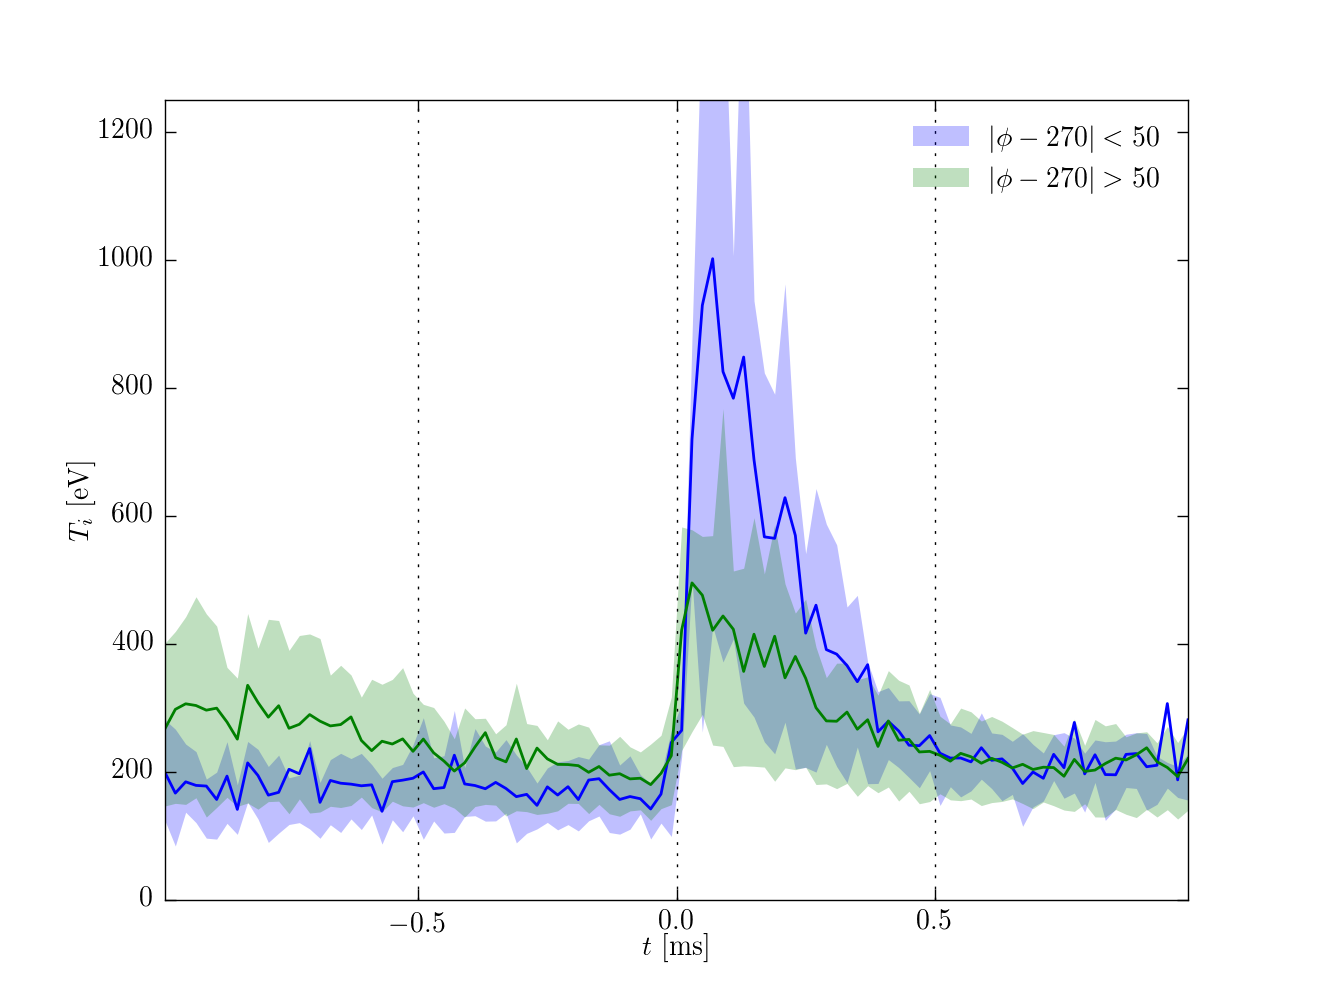
\includegraphics[width = 1.\linewidth]{./m0_and_impurity_heating/m0_no_delay.png}
	\caption{Ensemble $T_{C^{6+}}$ comparison between bursts near the location of observations. A) shows the comparison for $\rho/a = 0.75$ and B) shows the comparison for $\rho/a = 0.55$. Neither indicates any time delay associated with toroidal location.}\label{fig:m0_no_delay}
\end{figure}


An important observation resulting from the active measurements are high speed at which heating propagates around the machine. As can be seen in figure \ref{fig:m0_no_delay}, when the burst heating measurements are broken down into sub-ensembles separated by distance between the toroidal measurement location and the burst location, no delay is found. The charge exchange data is fitted at 50kHz, implying that any possible delay is smaller than 20$\mu s$. This indicates that the impurity heating is toroidally global. If we assume that the opposite is true, that the burst produces a local heating event located where the burst is located, then the toroidally local deposit of heat would need to travel to the other side of the device. For a very simple estimation of the time involved, the travel times of hypothetical deuterium ions at thermal velocity along equilibrium field line from one location to the direct opposite side of device toroidally are calculated for a range of $\rho$ near the reversal surface. This is presented in figure \ref{fig:heat_travel_time}. The actual thermal conduction time would be significantly longer than this as parallel conduction is slowed by collisions, and impurity thermal velocity is slower than deuterium. The delay of a toroially travelling heat pulse would be slower than 20$\mu s$, meaning that the observed heating is not a result of such a heat pulse, but the energy released through the m = 0 bursts travels around the device as EM waves/fluctuations and result in toroidally global (but radially local) impurity heating. The heating mechanism is not clear from this observation alone.

\begin{figure}
	\centering
	\includegraphics[width = 1.\linewidth]{./m0_and_impurity_heating/m0_travel_time.png}
	\caption{Estimated heat pulse travel time. It is evaluated for hypothetical deuterium ions at thermal velocity along equilibrium field line from one location to the direct opposite side of device toroidally.}\label{fig:heat_travel_time}
\end{figure}

The impurity heating associated with sawtooth events are known to be anisotropic, and the potential anisotropy of m = 0 induced impurity heating is investigated through passive IDS observations of C$^{4+}$ and C$^{2+}$ temperatures. The density profile of these two carbon charge states have limited radial extent, forming an emission 'shell'. A passive IDS view directly across the shell capture the perpendicular, and in ideal condition, a view directly tangential to the emission shell at the reversal surface would return the parallel temperature. In reality the passive measurements cannot be directly translated to perpendicular and parallel temperature, although it is sufficient to estimate anisotropy in past studies \cite{Anisotropy_papers}. Two emission shells are measured for anisotropy estimation. The C$^{2+}$ emission shell is located far out in the edge, outside of the reversal surface (at ~46cm -> $\rho/a = 0.9$) and it is extensively studied by T. Nishizawa during his drift wave work \cite{Nishizawa2018, Nishizawa2018b}. It also have a higher mass to charge ratio, which, according to theories developed for sawtooth crash heating, should correlate to more significant heating and anisotropy\cite{}. The C$^{4+}$ emission shell is somewhat broader but around the reversal surface. The measurement are done such that the two views are measured simultaneously, and thus, each burst in the ensemble contributes both ~$T_{\perp}$ and ~$T_{\parallel}$. The (approximately) parallel observation is taken from the inboard side of the device to reduce any effects from the increased wall integration during the burst, which primarily interacts with the outboard limiter. The results shows confusing contradiction. While both sets of measurements show anisotropy, the 'direction' of anisotropy is conflicting. The C$^{4+}$ measurement show $\Delta T_{\parallel} > \Delta T_{\perp}$, but the C$^{2+}$ measurement show $\Delta T_{\perp} > \Delta T_{\parallel}$. Additionally, the observed anisotropic heating associated with sawtooth events have the perpendicular direction being the strongly heated one, corresponding to expectations for possible heating mechanisms such as stochastic heating, or ion cyclotron damping. The strong parallel heating observed here with C$^{4+}$ does not have a ready made heating mechanism associated. However, these anisotropy arguments should be taken with a grain of salt as described above, as well as the fact that the emission shell location may move dramatically over the course of the observation period as sharp movements in flux surface and particle flux is expected for the burst. It would be more ideal to observe anisotropy through active CHERS measurement, but currently the CHERS toroidal view is not able to measure the radial region of interest. 

\begin{figure}
	\centering
	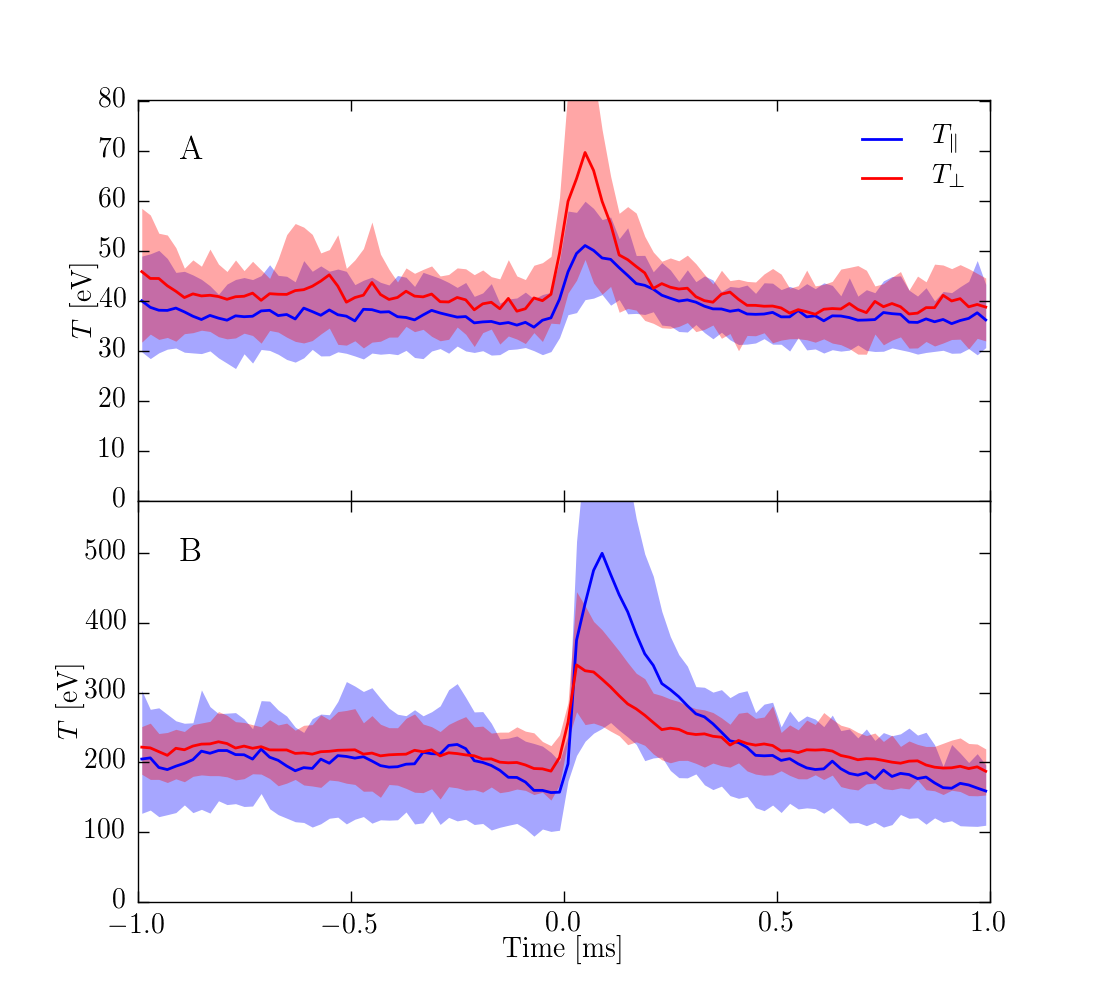
\includegraphics[width = 1.\linewidth]{./m0_and_impurity_heating/m0_anisotropy.png}
	\caption[Anisotropic impurity heating associated with m = 0.]{Anisotropic impurity heating associated with m = 0. Approximately perpendicular and parallel temperatures are measured by taking advantage of the emission shell geometry. Results are presented for A) C$^{2+}$ and B)  C$^{4+}$}\label{fig:m0_anisotropy}
\end{figure}

\section{Classical ion thermal model results of m = 0 bursts}

It is interesting to examine the equilibrium ion transport model response to a m = 0 -like heating event, through it is importantly to note that the model does not produce a direct comparison to observations as the model produces the response to direct majority ion heating. The zeroth order approximation involves simulating the burst heating by increasing the the \textit{ad hoc} term described in section \ref{sec:anomalous_heating} for a short duration (0.1ms) that corresponds to the typical burst duration. The magnitude of this increase is matched to the observed peak temperature at $\rho/a = 0.75$, and the model predictions are shown in figure \ref{fig:m0_model}. The characteristic time of the return to equilibrium as predicted by the forward model is noticeably longer than observations. Meaning the confinement of the carbon impurities are lower than that (expected) of the majority ion. However, assuming that m = 0 related impurity heating is through similar mechanisms to that present in sawtooth crashes, then it would be expected that the impurities experiences more heating than the majority ion. If that is the case, the observed T$_{C^{6+}}$ fall off would be determined primarily by the equilibration time with the majority ion, which is calculated to be ~0.3-0.5ms near the reversal surface for these plasma conditions. The observed equilibration time matches this time scale, but without direct measurement of majority ion temperature, it is not not possible to rule out other explanations. 

\begin{figure}
	\centering
	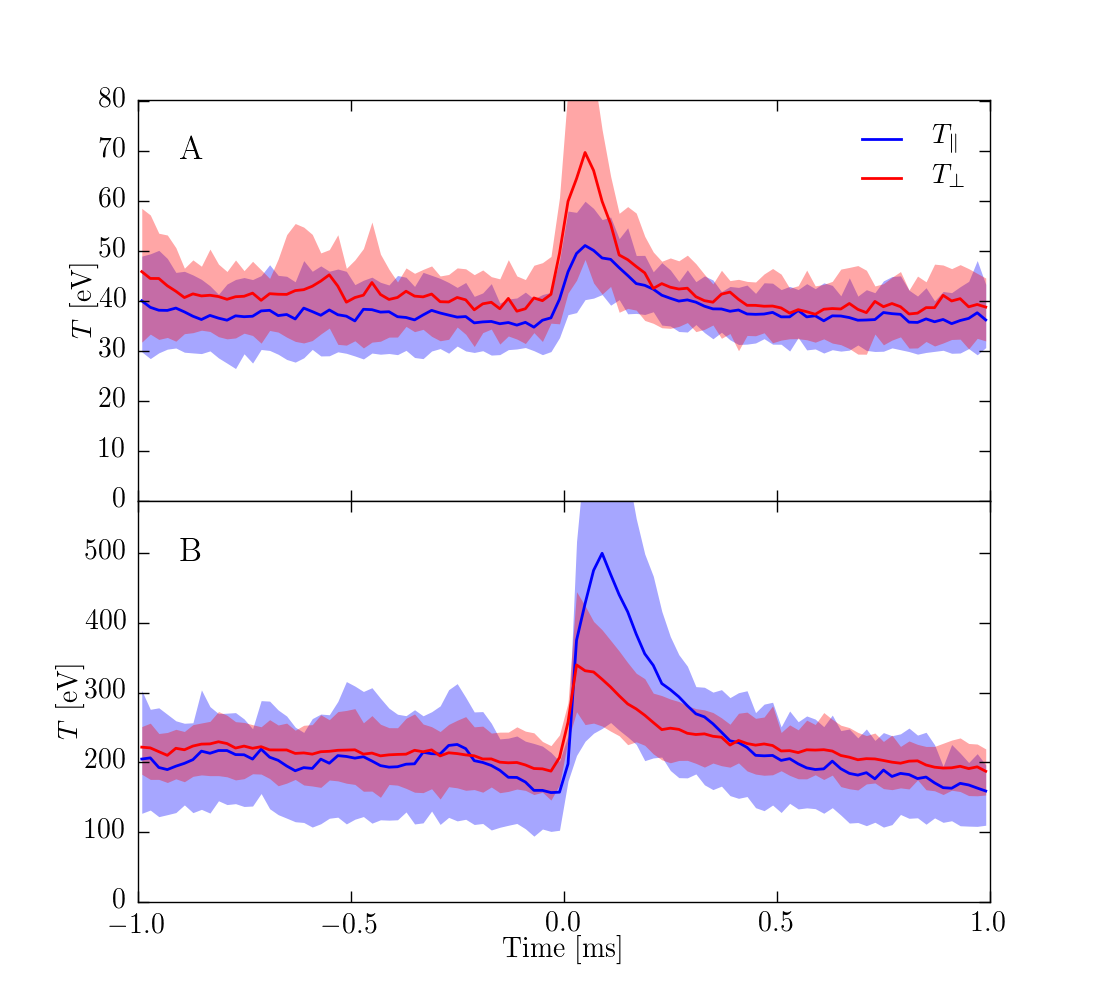
\includegraphics[width = 1.\linewidth]{./m0_and_impurity_heating/m0_anisotropy.png}
	\caption[Model response to m = 0 like heating to the majority ions.]{Model response to m = 0 like heating to the majority ions. The model input data is the same shot ensemble used for analysis in the previous chapter, with the exception of a short burst of extra \textit{ad hoc} heating. }\label{fig:m0_model}
\end{figure}

However, the heating response produced is radially located to the same locations as observations without additional adjustments to the radial profile of the \textit{ad hoc} heating term. Considering the fact that the tearing mode activity is reduced and not eliminated, it is tempting to speculate that the \textit{ad hoc} heating needed by the model during the temperature 